\section*{Preamble}
rationale, overview, co-authorship statement, ethics approval (if applicable)

\section*{Contents}

\begin{center}

\textbf{Inexpensive diffuse reflectance spectroscopy system for measuring changes in tissue optical properties}

Diana L. Glennie, Joseph E. Hayward, Daniel E. McKee, and Thomas J. Farrell

\textit{Department of Medical Physics and Applied Radiation Sciences, McMaster University, 1280 Main Street West, Hamilton, Ontario, L8S 1A8}

\textit{AND}

\textit{Department of Medical Physics, Juravinski Cancer Centre, 699 Concession Street, Hamilton, Ontario, L8V 5C2}

\end{center}

\noindent Journal of Biomedical Optics \textbf{19}(10), 105005 (October 2014).

\noindent \url{http://dx.doi.org/10.1117/1.JBO.19.10.105005}

\section*{Abstract}
The measurement of changes in blood volume in tissue is important for monitoring the effects of a wide range of therapeutic interventions, from radiation therapy to skin-flap transplants. Many systems available for purchase are either expensive or difficult to use, limiting their utility in the clinical setting. A low-cost system, capable of measuring changes in tissue blood volume via diffuse reflectance spectroscopy is presented. The system consists of an integrating sphere coupled via optical fibers to a broadband light source and a spectrometer. Validation data are presented to illustrate the accuracy and reproducibility of the system. The validity and utility of this \emph{in vivo} system were demonstrated in a skin blanching/reddening experiment using epinephrine and lidocaine, and in a study measuring the severity of radiation-induced erythema during radiation therapy.

\bigskip
\bigskip

\noindent \textcopyright 2014 Society of Photo-Optical Instrumentation Engineers (SPIE)

\section{Introduction}
The ability to quantify changes in the concentration of chromophores in the skin (particularly oxy- and deoxy-hemoglobin) in vivo and in real time has many applications in healthcare. For example, a complication of radiation therapy is radiation-induced erythema, which, if not monitored closely, can progress to painful moist desquamation.\cite{Hopewell1990,Russell1994,Nystrom2004,Fitzgerald2008} In photodynamic therapy, tissue oxygenation can be used to indicate treatment efficacy\cite{Woodhams2007} since oxygen is required for the activation of the cytotoxic photochemicals.\cite{Patterson1989a,Wilson2008} Finally, in plastic surgery, proper blood flow is integral for the success of free tissue transplants and is used to indicate whether or not a return to the operating room is necessary.\cite{Steele2011}

Several methods have been validated for measuring skin redness. In increasing complexity and accuracy they are visual assessment (with or without a color chart), colorimetry/photography, and spectroscopy.\cite{Agache2004} Although the visual assessment technique,\cite{Trotti2003} is the most common, it is qualitative in nature. Due to its subjective nature and the nonlinearity of human vision, it is highly prone to interobserver as well as intraobserver variations.\cite{Bodekaer2013} The subjectivity of this method can be minimized by the introduction of color charts; however, a very large number of color shades would be required to best account for the effect of pigmentation on the perceived redness. Despite these difficulties, visual assessment remains the gold standard for measuring skin redness.\cite{Basketter1997,Wengstrom2004}

Digital photography is usually approached as a two-dimensional implementation of colorimetry. In colorimetry, the color is quantified using a set of three specifically tuned color sensors (usually RGB) that represent the color using a standard color map, such as the L*a*b* system from the International Commission on Illumination (CIE).\cite{CI2012} Colorimetry (and digital photography) is made extremely difficult by the necessity to calibrate and standardize the results to allow for intermeasurement comparison (between days or between individuals).\cite{Jung2012} Following correct calibration, both methods are capable of detecting changes in blood and oxygen saturation but, since the relationship between the measured data and skin redness is not fully characterized, they are only capable of indicating whether the skin is more or less red in comparison to previous or baseline measurements.\cite{Kollias2002,Canning2009,Nishidate2011,Setaro2002}

Spectroscopy-based methods, such as reflectance spectroscopy and hyperspectral imaging, are the most complex of the methods used for measuring skin color.\cite{Zhang2005,Stamatas2008,Kollias2010,Yudovsky2010,Chin2012} Spectroscopy provides quantitative data across a range of wavelengths, allowing for different parameters to be extracted from its measurements, depending on the scope of the investigation and the apparatus used. User-friendly commercial models capable of monitoring relative erythema and tissue oxygen saturation are expensive and use single-use detection probes. For example, the T-Stat\textregistered (Spectros, Portola Valley, California) costs approximately \$25,000 US.\cite{Fox2012} Cheaper models are less user-friendly and mostly only provide a single value for oxygen saturation. As a result, these systems are primarily used by highly trained investigators at research institutions and are rarely utilized in a typical clinical setting where they could be used routinely and would prove most beneficial.

In order to facilitate the translation of spectroscopy systems from the research laboratory to the routine clinical setting for the use on human skin in vivo, an economic integrating sphere-based diffuse reflectance spectroscopy (DRS) unit was developed and characterized. The system designs and specifications will be outlined. To illustrate the validity and utility of the assembled system, the results of two ongoing clinical studies measuring erythema under different conditions will be presented.

\section{Design of the Total DRS System}
Simply, the total DRS system consists of a white light source coupled to an integrating sphere via an optical fiber. A second detection optical fiber directs the reflected light to a spectrometer. The spectrometer is controlled by a computer on which the required processing software was installed. A schematic of the system design is shown in Figure~\ref{fig:p1-sys_diagram}. A detailed description of the selection of each component is presented below.

\begin{figure}
	\centering 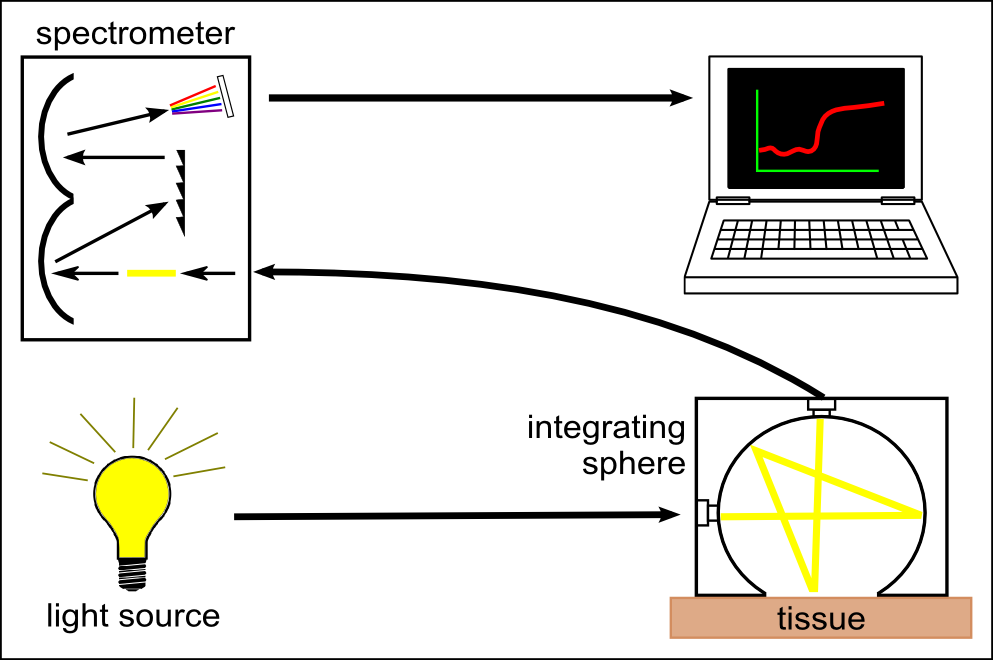
\includegraphics[width=0.6\textwidth]{figures/p1-sys_diagram.png}
	\caption[System schematic]{\label{fig:p1-sys_diagram}A schematic of the measurement system (not to scale). The light source is connected to the side port of the integrating sphere. Light collected through the overhead port is detected by the spectrometer and processed by the laptop.}
\end{figure}

\subsection{Light Source}
Oxy- and deoxy-hemoglobin have spectral absorption features within the visible light range.\cite{Young1997,Lister2012} Therefore, a light source encompassing this range, without any narrow bandwidth spectral excitation features, is required. In addition, a stable output over the measurement period (minutes to hours) is required for proper reflectance calculation. An Oriel 77501 Radiometric Fiber Optic Source (Newport, Irvine, California) was chosen with a 100 W quartz tungsten halogen lamp to produce a highly stable output within the visible-NIR wavelength range that can be easily coupled to an optical fiber. It also has an adjustable iris to allow for output optimization.

\subsection{Spectrometer and Optical Fibers}
The spectrometer must be capable of detecting light with high sensitivity across the visible spectrum. It must also have sufficient spectral resolution to allow for the differentiation between the spectral features of oxy- and deoxy-hemoglobin (<13 nm for oxy-hemoglobin). An ideal spectrometer would also be small for ease of portability.

The S2000 Miniature Fiber Optic Spectrometer from Ocean Optics (Dunedin, Florida) was chosen for this system. It has a wavelength range of 340 to 1000 nm and a dynamic range of 2000 for a single scan. The 2048-element linear CCD-array results in a pixel width of approximately 0.35 nm and the integration time can range from 3 ms to 60 s. Its small size (<150 mm cube) allows for easy transportation between clinical sites.

The fiber optic connector specifications for the Ocean Optics spectrometer are for an SMA 905 to single-strand 0.22 NA optical fiber. The optical fiber acts in place of a slit in the spectrometer’s hardware. A relatively large fiber core of 400 \si{\um} was chosen to maximize light collection. This resulted in spectral resolution of 10 nm as determined from the measurement of a mercury–argon calibration source (HG-1 Mercury Argon Calibration Source, Ocean Optics, Dunedin, Florida). The effect of this spectral resolution on the reflectance spectrum analysis is described in Section~\ref{sec:ei_analysis}. The final criterion for the fibers was high transmission in the visible spectrum. Two such fibers, with a wavelength range between 400 and 2200 nm, were purchased from Thorlabs (Newton, New Jersey).

\subsection{Integrating Sphere}
The size of the integrating sphere is dictated by its use to measure light reflectance from human skin. As such, the integrating sphere should be relatively small (on the order of 5 to 10 cm in diameter) so that it can fit onto the various curves of the human body. A small sphere would also be easier to maneuver and keep stationary, resulting in more stable measurements.

The size of the measurement port of the sphere should be sufficiently large that local inhomogeneities in the measurement area (such as small freckles or hairs) do not overwhelm the result, but should result in the sphere’s port fraction (the ratio of the total port area to the total internal surface area of the sphere) falling between 2\% and 5\%.\cite{Hanssen2002} For the range of sphere sizes suggested above, the port diameter would fall somewhere within 1.5 to 5 cm.

The sphere should also have a high internal reflectance (greater than 94\%) and produce a uniform light field at the measurement port.\cite{Labsphereb,Labspherea,Labsphere} If the input light is directly incident on the detection port, the sphere should include a baffle, blocking this path. For spheres of the size used in this experiment, baffles should be avoided when possible as they disrupt the internal surface of the sphere, reducing the uniformity of the illumination within the sphere.

The integrating sphere was made from a cube of Spectralon\textregistered (Labsphere\textregistered, North Sutton, New Hampshire) with side lengths of 2 in. (50.8 mm). The cube was bisected and a hemispherical cavity was machined into both halves using a 1\textonequarter in. (31.75 mm) ball-end mill. The bottom of one of these halves was milled down, creating a port measuring 15.2 mm in diameter. The parts were assembled to form the sphere and holes were drilled through the center of the unmilled half as well as through one side at the junction to accommodate SMA 905 connectors which would become the detection and illumination ports, respectively (see Figure~\ref{fig:p1-intsphere_schematic}).

\begin{figure}
	\centering 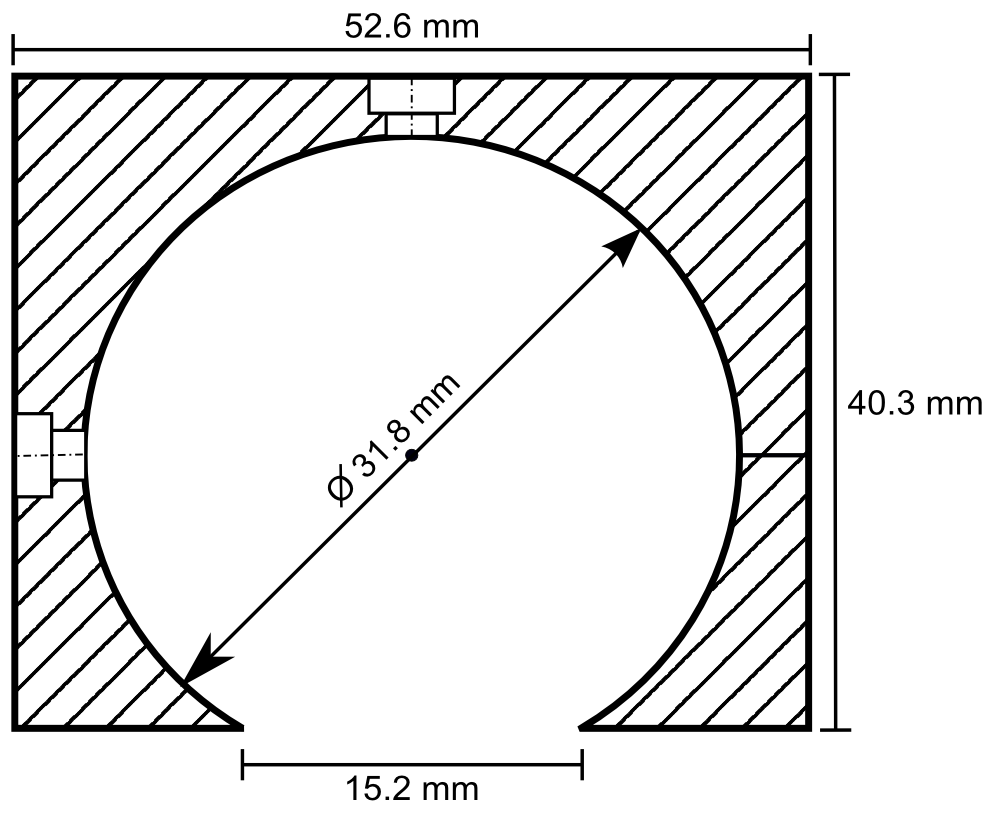
\includegraphics[width=0.5\textwidth]{figures/p1-intsphere_schematic.png}
	\caption[Cross-sectional diagram of the integrating sphere]{\label{fig:p1-intsphere_schematic}A cross-sectional diagram of the integrating sphere. The block of Spectralon\textregistered used to make the sphere is bisected before processing and then reattached to form the sphere.}
\end{figure}

\subsection{Implementation Costs}
The specifications for each individual component have some flexibility; therefore, a DRS system can be built within a wide range of costs while still achieving the same measurement results.

In choosing the light source, it is only important that it covers the desired wavelength range and be stable to within 1\%. Although a uniform spectral output is ideal to keep the signal uncertainty relatively constant, it is not necessary. A quartz tungsten halogen lamp provides smooth spectral features and high output powers; however, a less expensive alternative would be a white LED. These provide excellent illumination and are relatively stable, although they do have an emission peak in the blue region (\textasciitilde465 nm).

Integrating spheres can be purchased from an optical device supplier; however, spheres can be built for costs as low as \$100 US by obtaining a suitable block of Spectralon. Since the sphere is not being used for radiometric purposes, it can deviate from an ideal integrating sphere and still provide an accurate reflectance measurement. Spheres can also be constructed by vacuum-forming plastic styrene about a spherical mold and coating the inside with barium sulfate paint.\cite{Glennie2009}

The most expensive piece of equipment component is the spectrometer, and its price will depend on the detection sensitivity and grating size. The average cost for a common fiber-based spectrometer is around \$2000 US. Although not recommended, spectrometers can also be built cheaply if necessary.\cite{Sumriddetchkajorn2012}

The computer must be able to interface with the spectrometer and run the necessary software. Therefore, an inexpensive netbook or laptop will be sufficient. Optical fibers are uniformly priced in the market and will contribute very little to the total cost of the system.

A list of itemized expenses is shown in Table 1, assuming new materials were required. For comparison, a hand-held colorimeter is available for \$6000 US from Derma Spectrometer (MIC Global, London, United Kingdom).

\begin{table}[h]
	\centering
	\caption{Cost estimates for the DRS system. Listed prices are based on the purchase of new material.}
	\label{my-label}
	\begin{tabular}{lcc}
		\toprule
		\multirow{2}{*}{Component} & \multicolumn{2}{c}{Pricing (USD)} \\ \cmidrule(l){2-3} 
		& Low             & High            \\ \midrule
		Light source               & \$100           & \$500           \\
		Integrating sphere\qquad\qquad         & \$100           & \$1500          \\
		Spectrometer               & \$500           & \$3000          \\
		Computer                   & \$250           & \$500           \\
		Connection cables\qquad\qquad          & \$100           & \$200           \\
		\textbf{Total}             & \textbf{\qquad\$1050\qquad} & \textbf{\qquad\$5700\qquad} \\ \bottomrule
	\end{tabular}
\end{table}

\section{Procedure and Performance}

\subsection{Integrating Sphere Configuration}
The optical fibers are connected to the integrating sphere following a d/0\degree (diffuse illumination/direct detection) geometry such that the input light is first incident on the sphere wall before encountering the tissue surface and the output fiber is directly across from the measurement port (as shown in Figure~\ref{fig:p1-sys_diagram}. In this geometry, the sample is more uniformly illuminated compared with a 0\degree/d geometry due to the multiple reflections of the light prior to exiting the sphere at the tissue. In addition, since the illumination is diffuse rather than normally incident, the penetration of light is more superficial due to the oblique entrance angle (average 55\degree). Thus, a greater percentage of spectroscopic information originates from the upper layers of skin where the chromophores of interest are located. Due to the small size of this integrating sphere, a baffle was not used. The geometry and the detector fiber acceptance angle (0.22 NA) allowed only light that was specularly or diffusely reflected from the tissue surface to be collected.

\subsection{Calculating Spectral Reflectance}
The spectral reflectance of a tissue sample was normalized by dividing the spectral count rate with the detection port on the tissue, $S_t(\lambda)$, by the spectral count rate from a highly reflecting standard, $S_{norm}(\lambda)$. Both of these were adjusted by subtracting the background signal rate, $S_{bg}(\lambda)$, so that the modified total diffuse reflectance, R*m(?), is given by

\begin{equation}
	R_m^\ast(\lambda)=\frac{S_t(\lambda)-S_{bg}(\lambda)}{S_{norm}(\lambda)-S_{bg}(\lambda)}.
\end{equation}

Normalizing to a reflectance standard eliminates the need to correct the measured signal rate for the system spectral response.

A 99\% reflectance standard (SRS-99-010, Labsphere, North Sutton, New Hampshire) was used as the normalization standard while a 2\% reflectance standard (SRS-02-010, Labsphere, North Sutton, New Hampshire) was used for the background. The 2\% standard was used instead of directing the detection port into a dark room in order to avoid changes in ambient lighting conditions, should the system be used in different locations which would affect the calculated reflectance. This substitution did not affect the accuracy or precision of the measurement. If reflectance standards are not available, a piece of thick, matte black cloth may be substituted for the 2\% standard, and a piece of high diffusely reflective material such as a piece of Spectralon or a flat surface coated with barium sulfate may be substituted.

For each spectral count rate measurement, the integration time was set such that the maximum intensity was approximately 90\% of the dynamic range. This allowed for optimal precision while ensuring that the signal would not saturate. Five measurements were averaged to further reduce the noise. The averaged measurements were converted into a count rate by dividing by the integration times.

\subsection{Sphere Preparation}
The measurement port of the integrating sphere was covered with a sheet of occlusive dressing (Tegaderm\texttrademark film, 3M Health Care, St. Paul, Minnesota) in order to prevent dirt and other material from contaminating the inside of the sphere. A new sheet was applied for each patient before any measurements to ensure sterility. The dressing was left on for the normalization and background measurements and, therefore, did not modify the resulting reflectance. Reflectance measurements were performed on calibrated diffuse reflectance standards ranging from 2\% to 99\% (RSS-08-010, Labsphere, North Sutton, New Hampshire) with the dressing in place and removed. Both sets of measurements showed no measurable difference.

\subsection{Correcting for Single Beam Substitution Error}
Single beam integrating spheres used for reflectance spectroscopy suffer from single beam substitution error\cite{Springsteen1998,Labspherec} due to the decrease of the total flux within the sphere when the normalization plate is replaced with the sample. This can be corrected using Equation~\ref{eq:sbse}. The parameters (a, b, c), as a function of wavelength, were determined empirically by measuring the calibrated reflectance standards described in the previous section and developing a relationship between the measured and calibrated reflectances (represented by $R_m^\ast$ and $R_m$, respectively), based on the fraction of reflected light. If reflectance standards are not available, Intralipid\texttrademark (Baxter, Deerfield, Illinois) and India ink liquid phantoms can be used as they have well-characterized extinction coefficients.\cite{Flock1992,Madsen1992}

\begin{equation}
\label{eq:sbse}
	R_m = \frac{aR_m^\ast + b}{R_m^\ast + c}
\end{equation}

These data were fit using a nonlinear least-squares algorithm at each of the wavelengths. A typical fit for a single wavelength is shown in Figure~\ref{fig:p1-sbse_cf}. This correction was applied to the modified total diffuse reflectance, resulting in a corrected total diffuse reflectance ($R_m$). A set of colored diffuse reflectance standards (CSS-04-010, Labsphere, North Sutton, New Hampshire) were measured and, following correction, the measured reflectance was within 0.01 of the calibrated reflectance specified by the supplier (Figure~\ref{fig:p1-colored_refl}).

\begin{figure}
	\centering 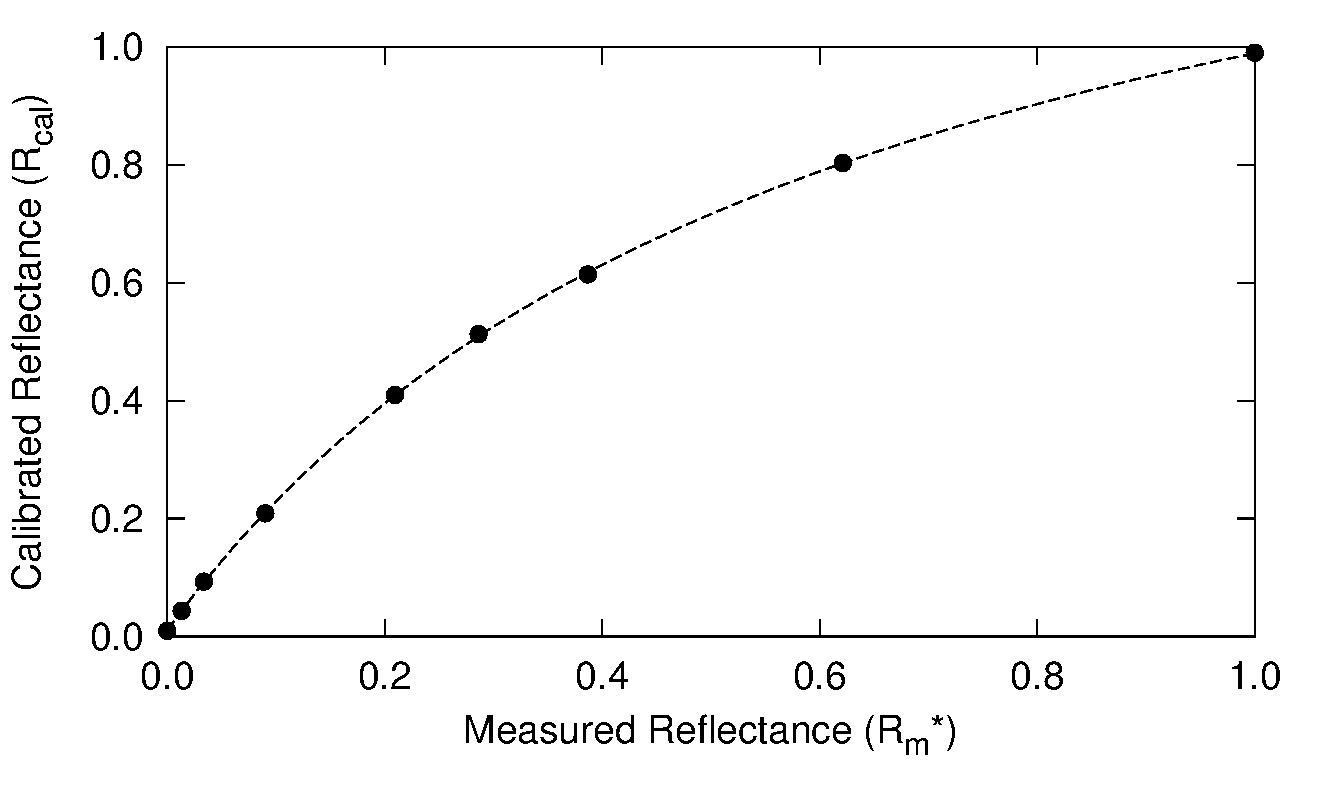
\includegraphics[width=0.7\textwidth]{figures/p1-sbse_cf.png}
	\caption[Single-beam substitution error correction curve text]{\label{fig:p1-sbse_cf}The integrating sphere calibration curve at 600 nm. The fitted function corrects the measured reflectance for single-beam substitution error. The dots are the calibrated and measured reflectance pairs and the dashed line is the fit to these data.}
\end{figure}

\begin{figure}
	\centering 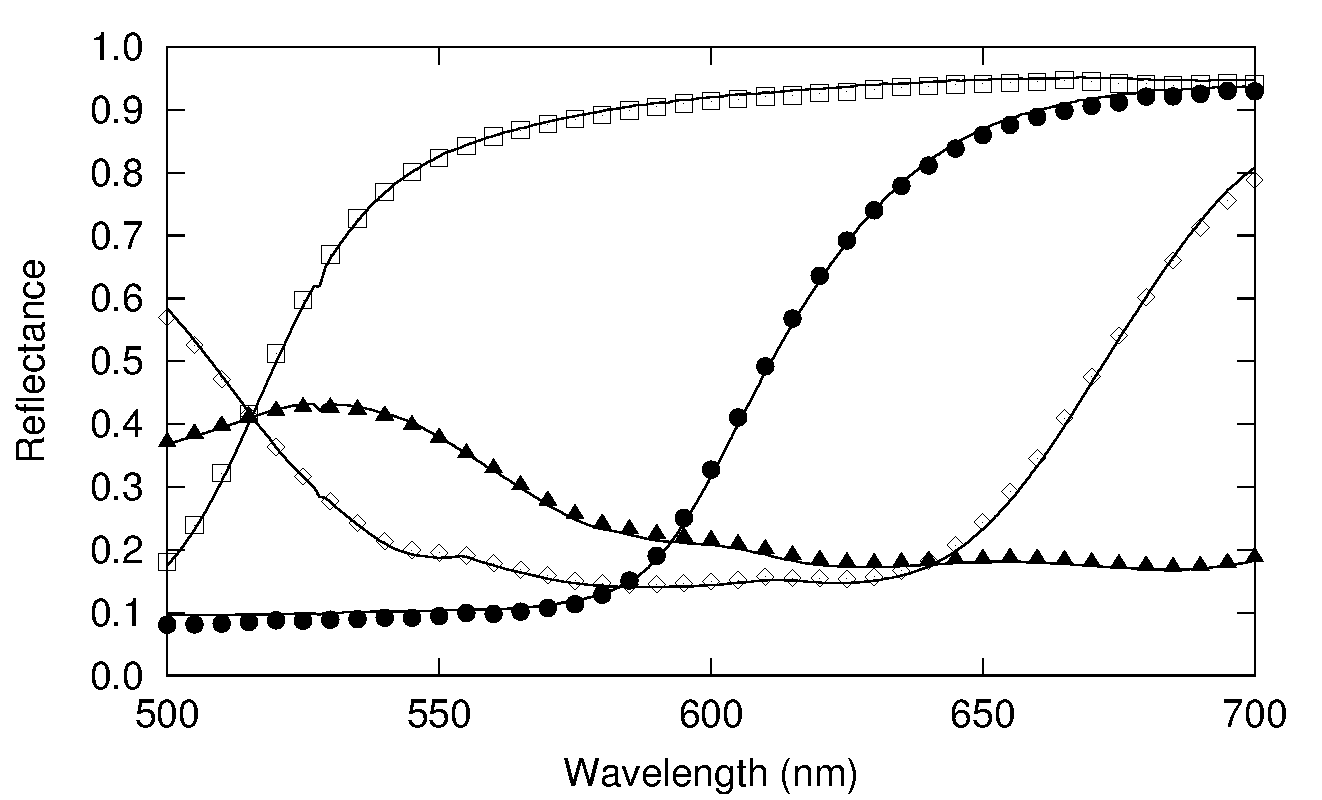
\includegraphics[width=0.7\textwidth]{figures/p1-colored_refl.png}
	\caption[Measured and calibrated reflectance spectra]{\label{fig:p1-colored_refl}The measured (symbols) and calibrated (lines) reflectance spectra for a set of four colored diffuse reflectance standards: red (CIRCLE), yellow ($\square$), green (TRIANGLE), and blue ($\diamond$). Correction for the single-beam substitution error brought the measured reflectance values to within 0.01 of the calibrated reflectance specified by the supplier.}
\end{figure}

\subsection{Reflectance Measurement Reproducibility}
The reproducibility of the system was tested using the green reflectance standard (SCS-GN-010) because it had reflectance similar to human skin and spectral features in the same region as hemoglobin. Reflectance was measured every day for 30 days and the standard deviation across the 500 to 700 nm spectral region never exceeded 1\%. As expected, it varied with the spectral reflectance of the reflectance standard (i.e., the uncertainty was lower when the reflectance/signal was higher). Reproducibility measurements were also performed on human skin and they had a similar result.

\section{Experimental Validation}

\subsection{Study Overviews}
In order to demonstrate the use and validity of the DRS system, sample data from two ongoing erythema studies are presented. In the first study, erythema and skin blanching were induced via subcutaneous injection of lidocaine (a vasodilator and anesthetic) with or without epinephrine (a vasoconstrictor) over the deltoid muscles of volunteers’ upper arms. The aim of this study was to determine the time to maximal effect of injected epinephrine. In the second study, serial skin reflectance measurements were taken on head and neck cancer patients undergoing intensity-modulated radiation therapy (IMRT). The goal of this study was earlier detection of radiation-induced erythema compared with visual assessment methods. Both studies received Hamilton Health Sciences Research Ethics approval.

\subsection{Erythema Index Analysis}
\label{sec:ei_analysis}
The measured reflectance spectra were processed using the Dawson erythema index (EI).\cite{Dawson1980} This model was chosen because of its wide acceptance and use (over 280 citations to date),\cite{Riordan2001} as well as its straight-forward calculation method. Briefly, the EI is the area under the curve of the log of the inverse reflectance spectrum between 510 and 610 nm (encompassing the absorption features of oxy- and deoxy-hemoglobin). The influence of melanin in the EI can be approximately corrected using reflectance data between 650 and 700 nm (EI). For serial measurements on an individual, a relative erythema index (EI\textsubscript{r}) can also be calculated. Simply, a baseline EI\textsubscript{c} is obtained either at time zero or at a nearby reference location. This is subtracted from EI\textsubscript{c} values measured at later time points such that, in the absence of changes in hemoglobin, EI\textsubscript{r} would be zero.

The 10 nm FWHM spectral resolution of the system has the effect of broadening spectral features in the measured reflectance. Although this would be problematic for narrow features, the absorption features in the hemoglobin spectra are very broad and were not strongly affected. To verify the effect on the EI, spectra derived from the literature\cite{Jacques1998} were convolved with a 10 nm FWHM Gaussian function and the EI calculated before and after. Small differences in the calculated EI were noted (data not shown), however changes in EI with respect to an increase or decrease in hemoglobin were insensitive to the spectrometer’s spectral resolution.

\subsection{Study Results}
In the first study, the reflectance was measured serially for 2 h following the injection of lidocaine (with or without epinephrine) and the measurements were processed to calculate the EIr as a function of time. A time course for one volunteer is shown in Figure~\ref{fig:p1-lido_epi} along with the reflectance spectra at specific time points. For both injections, there was a rapid increase in the EI\textsubscript{r} indicating an increase in the hemoglobin content. The combined lidocaine and epinephrine injection then decreased to a minimum EI\textsubscript{r} of approximately -16 at the 22 min mark indicating a reduction in hemoglobin content. An analysis of the EI\textsubscript{r} for all subjects indicated that the maximum epinephrine-induced blanching occurred approximately 25 min following injection, after which surgical incision may commence.\cite{McKee2013}

\begin{figure}
	\centering 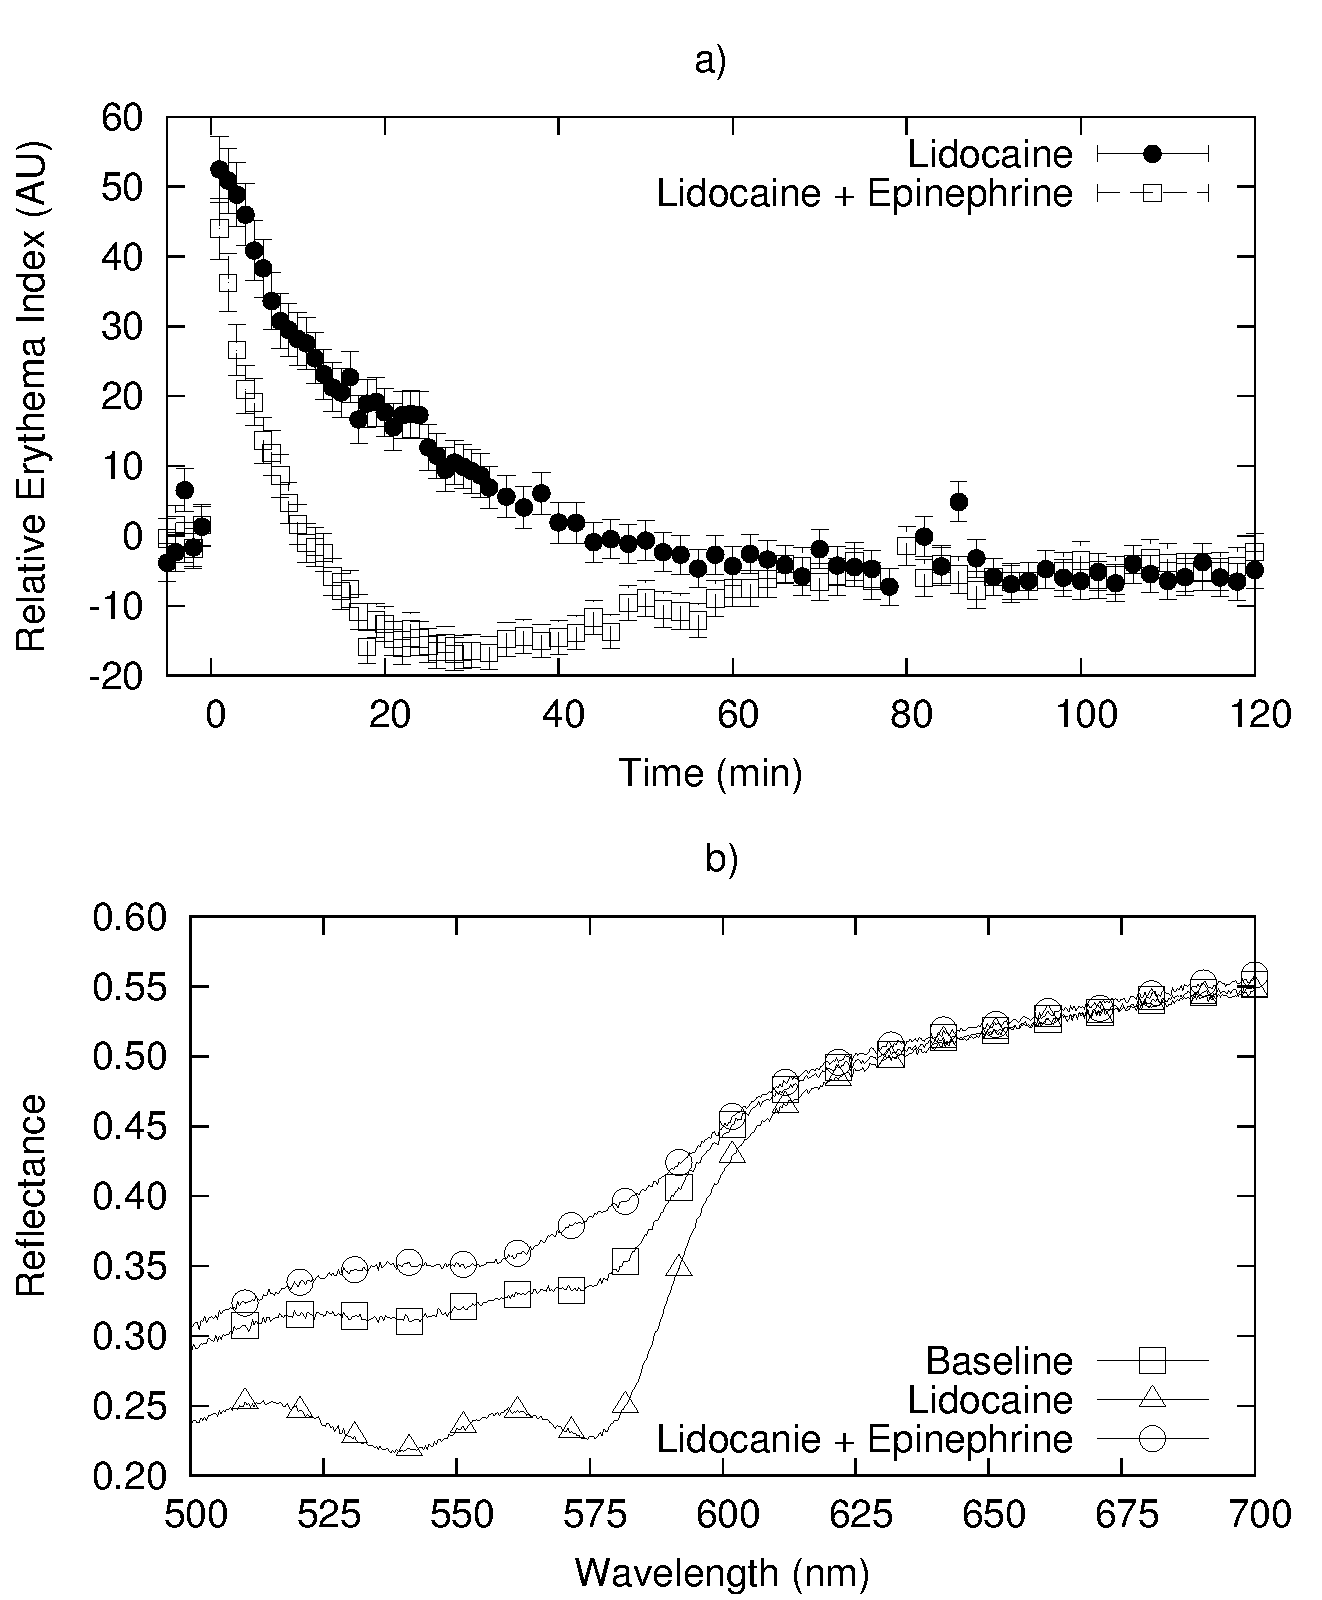
\includegraphics[width=0.7\textwidth]{figures/p1-lido_epi.png}
	\caption[Sample time course for lidocaine \& epinephrine]{\label{fig:p1-lido_epi}(a) A sample time course for one volunteer in the study involving lidocaine and epinephrine. (b) Full reflectance spectra from before injection ($\square$), 1 min following the injection of lidocaine alone ($\triangle$), and 26 min following the injection of lidocaine and epinephrine ($\bigcirc$).}
\end{figure}

In the second study, the reflectance was measured daily over the course of the patients’ head and neck IMRT treatments. During this study, it was necessary to have multiple investigators operate the DRS system. This requirement illustrated the ease of training associated with the system, as all investigators were capable of properly using the system following a short 15 min tutorial. Greater variation was observed in the daily measurements compared with the short-term measurements of the first study (see Figure~). The EI\textsubscript{r} was not calculated because the baseline consisted of a single measurement. The variation is the result of daily changes such as time of day and patient temperature.\cite{Fullerton1996} An increase in EI\textsubscript{c} was observed over the course of the 35 days. Erythema was first visually diagnosed on day 18 of treatment. This study is ongoing.

\begin{figure}
	\centering 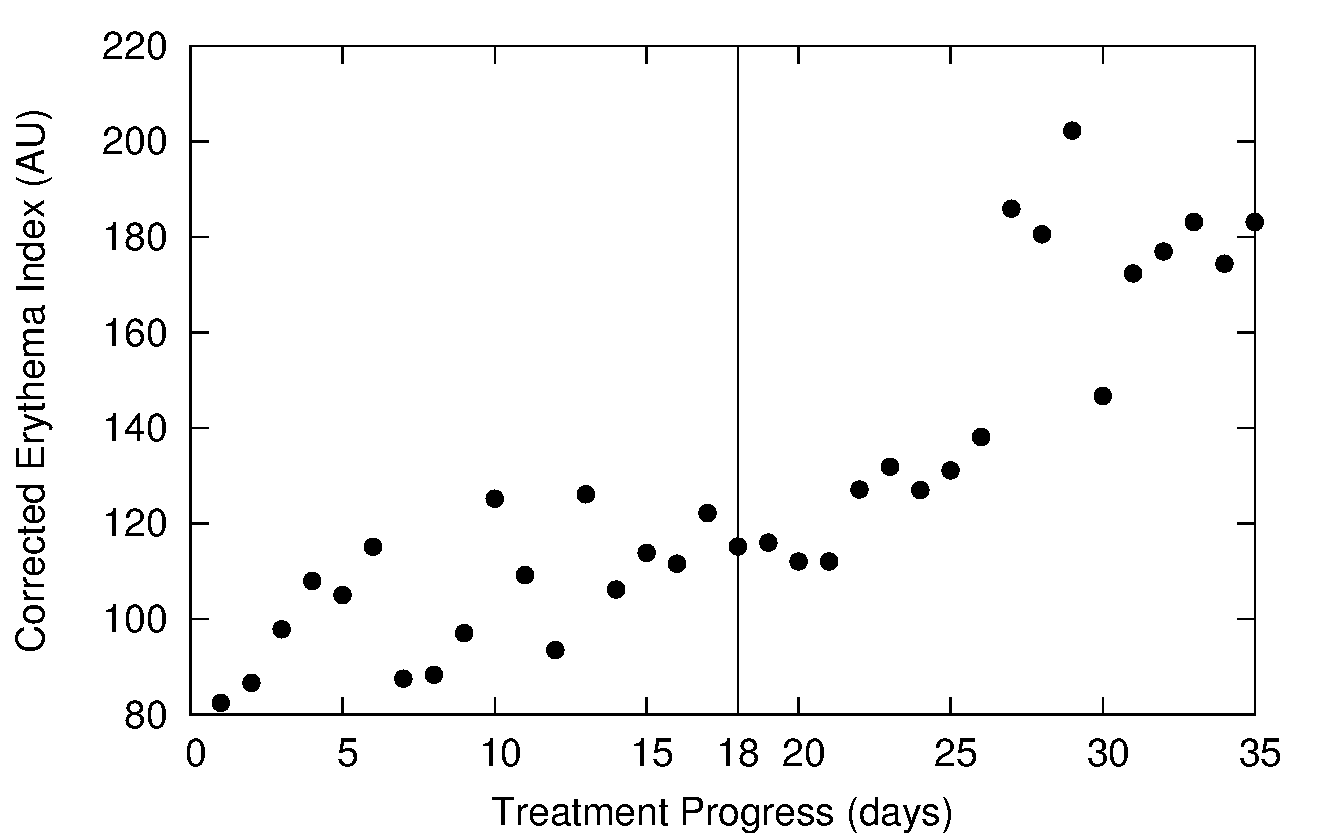
\includegraphics[width=0.7\textwidth]{figures/p1-cor_ei.png}
	\caption[Corrected erythema index for IMRT cancer patient]{\label{fig:p1-cor_ei}Corrected erythema index for a head and neck IMRT cancer patient. Daily measurements were taken over the course of treatment. Erythema was not visually noted until day 18.}
\end{figure}

\section{Discussion}
This paper illustrates two clinical applications of a DRS system. These results demonstrate that a low-cost spectroscopy system is capable of measuring spectral changes in reflectance due to changes in the concentration of hemoglobin. These changes were quantified using the Dawson EI. The system is easy to operate and yields valuable clinical data with little training required. The system described here may be found to have a wide range of clinical assessment roles, which would make it an even more useful tool for health care practitioners. However, since the system collects a full spectrum, it is capable of generating much more valuable information than just a single EI value. For example, correcting for background chromophores is only approximate and any changes over the measurement period could register as incorrect increases or decreases in skin redness. An alternative modeling approach using a spectrally constrained diffuse reflectance model to fit the measured reflectance spectrum with concentrations of the major tissue chromophores may be advantageous. This will allow for the detection of skin color changes in reference to their responsible chromophore, but would require the measured spectrum to be extremely accurate and precise.

One of the limitations of this spectroscopy system is that the signal is normalized using a highly scattering Spectralon\textregistered standard. In comparison, human skin is much less scattering and therefore the true reflectance is under-represented due to scattering losses. These scattering losses are not large but, since they vary with the tissue optical properties, they would need to be accounted for in a spectrally dependent model.

This paper presents a low-cost, user-friendly DRS system for measurement of changes in skin hemoglobin concentration. The performance of the system was characterized in terms of wavelength accuracy and measurement stability, uncertainty, and reproducibility. The validity and utility of the system were demonstrated through a skin reddening/blanching experiment and a radiation-induced erythema study, followed by analysis with a simple erythema model. Further uses of the system have yet to be investigated.

\section*{Acknowledgments}
The authors would like to thank Kevin R. Diamond and Gabriel A. Devenyi for their assistance in the preparation of this paper. This work was financially supported by the Natural Sciences and Engineering Research Council of Canada.